%% vim:ft=tex
\documentclass[chapter=TITLE,section=Title,espaco=duplo,tocpage=plain,appendix=Name,floatnumber=continuous]{abnt}
\usepackage{hyperref}
\usepackage[utf8]{inputenc}
\usepackage[brazil]{babel}
\usepackage[alf]{abntcite}
\usepackage{mdwlist}
\usepackage{dsfont}
\usepackage{graphicx}
\usepackage[small]{caption}
\usepackage{wrapfig}
\usepackage{setspace}
\usepackage{subfigure}
\usepackage{boxedminipage}

%% xunxo especial para seguir as normas da UTP
\usepackage{xunxos-utp}

%% informações sobre o trabalho
\autor{Nicolai Nicolaiev}
\coautor{Fulano Fulanowsky}
\titulo{Um exemplo de trabalho em \LaTeX{}}
\comentario{Trabalho de Conclusão de Curso apresentado ao Curso de Bacharelado
em Ciência da Computação, da Faculdade de Ciências Exatas da Universidade
Tuiuti do Paraná, como requisito parcial para a obtenção do grau de Bacharel em
Ciência da Computação.}
\instituicao{Universidade Tuiuti do Paraná}
\orientador{Parararan Parararanavam}
\local{Curitiba}
\data{2010}

\begin{document}
%% xunxos-utp.sty
%% Copyright 2010 Bogdano Arendartchuk <bhdn@ukr.net>
%
% This work may be distributed and/or modified under the
% conditions of the LaTeX Project Public License, either version 1.3
% of this license or (at your option) any later version.
% The latest version of this license is in
%   http://www.latex-project.org/lppl.txt
% and version 1.3 or later is part of all distributions of LaTeX
% version 2005/12/01 or later.
%
% This work has the LPPL maintenance status `maintained'.
% 
% The Current Maintainer of this work is M. Y. Name.
%
% This work consists of the files xunxos-utp.sty and xunxos-utp-doc.tex.
%
\renewcommand{\figurename}{FIGURA}
\renewcommand{\tablename}{TABELA}
\citeoption{minhasopcoes}
\nohyphens


%%\capa
%%\folhaderosto
\UTPCapa
\UTPFalsaFolhaDeRosto
\UTPFolhaDeRosto

\begin{resumo}
As experiências acumuladas demonstram que a contínua expansão de nossa
atividade afeta positivamente a correta previsão das novas proposições. Do
mesmo modo, a valorização de fatores subjetivos causa impacto indireto na
reavaliação dos paradigmas corporativos. Percebemos, cada vez mais, que o
fenômeno da Internet ainda não demonstrou convincentemente que vai
participar na mudança das diretrizes de desenvolvimento para o futuro. A
prática cotidiana prova que a determinação clara de objetivos talvez venha
a ressaltar a relatividade das formas de ação.

Palavras-chave: fermento; sal; açúcar; linhaça
\end{resumo}

\listoffigures
\listoftables
\listadequadros
\sumario

\chapter{INTRODUÇÃO}

As experiências acumuladas demonstram que a contínua expansão de nossa
atividade afeta positivamente a correta previsão das novas proposições. Do
mesmo modo, a valorização de fatores subjetivos causa impacto indireto na
reavaliação dos paradigmas corporativos. Percebemos, cada vez mais, que o
fenômeno da Internet ainda não demonstrou convincentemente que vai
participar na mudança das diretrizes de desenvolvimento para o futuro. A
prática cotidiana prova que a determinação clara de objetivos talvez venha
a ressaltar a relatividade das formas de ação. 

\chapter{REVISÃO DA LITERATURA}

Segundo~\cite{joachims1998text}, a natureza do aprendizado estatístico não
deve-se apenas aos problemas da humanidade.

Porém, segundo~\cite{vapnik2000nature}, nada disso é verdade.

Pensando mais a longo prazo, a expansão dos mercados mundiais pode nos
levar a considerar a reestruturação de todos os recursos funcionais
envolvidos. Acima de tudo, é fundamental ressaltar que o aumento do diálogo
entre os diferentes setores produtivos auxilia a preparação e a composição
das diversas correntes de pensamento. Todavia, a execução dos pontos do
programa acarreta um processo de reformulação e modernização da gestão
inovadora da qual fazemos parte. Ainda assim, existem dúvidas a respeito de
como a necessidade de renovação processual prepara-nos para enfrentar
situações atípicas decorrentes dos modos de operação convencionais. A nível
organizacional, a competitividade nas transações comerciais exige a
precisão e a definição de alternativas às soluções ortodoxas.

E em imagens, porém,~\cite{semolini2002support} afirma que generalização
para duas dimensões para uma matriz $p$ de tamanho $n \times n$:
\begin{equation}
G_{ij} = \frac{1}{\sqrt{2n}} C_i C_j \sum_{x=0}^{n-1} \sum_{y=0}^{n-1}
         p_{xy} \cos{ \left ( \frac{(2y + 1) j \pi}{2n} \right ) }
              \cos{ \left ( \frac{(2x + 1) i \pi}{2n} \right ) }
\label{eq:dct_duas}
\end{equation}

\section{ESTE É O TÍTULO DESTA SEÇÃO}

Caros amigos, o comprometimento entre as ontologias apresenta tendências no
sentido de aprovar a manutenção das múltiplas direções do ponto de
transcendência do sentido enunciativo. Por outro lado, a complexidade dos
estudos efetuados cumpre um papel essencial na formulação do gênio grego
fundado na poesia homérica. Assim como indicado dela definição
\ref{eq:dct_duas}.  Assim mesmo, a estrutura atual da ideação semântica
pode nos levar a considerar a o \textit{merge} na \textbf{reestruturação}
da definição espinosista de substância. Neste sentido, existem duas
tendências que coexistem de modo heterogêneo, revelando o novo modelo
estruturalista aqui preconizado auxilia a preparação e a composição das
posturas dos filósofos divergentes com relação às suas atribuições.
Contudo, a crítica contundente de Deleuze/Guatarri - dupla implacável - nos
mostra que a indeterminação contínua de distintas formas de fenômeno
garante a contribuição de um grupo importante na determinação das novas
teorias propostas.

\begin{figure}[h!]
  \centering
  
\includegraphics[width=0.5\textwidth]{eagle.jpg}
  \caption[Uma retumbante águia]{Veja, uma águia e seu amigo.}
  \fonte{Wikipédia Commons, 2010}
\end{figure}

O incentivo ao avanço tecnológico, assim como a hegemonia do ambiente
político não pode mais se dissociar das condições inegavelmente
apropriadas. Gostaria de enfatizar que a constante divulgação das
informações oferece uma interessante oportunidade para verificação dos
relacionamentos verticais entre as hierarquias. O empenho em analisar a
mobilidade dos capitais internacionais é uma das consequências dos métodos
utilizados na avaliação de resultados \cite{semolini2002support}.

\begin{table}[h!b!p!]
\centering
\begin{tabular}{lll}
\hline
Alphabet Character & Vowel & Number \\
\hline
A & Yes & 1 \\
B & No & 2 \\
C & No & 3 \\
\hline
\end{tabular}
\caption{Uma super tabela}
\label{tab:seila}
\end{table}

De acordo com as idéias de Deleuze como na tabela ~\ref{tab:seila}, a crescente
influência da mídia acarreta um processo de reformulação e modernização das
diversas correntes de pensamento.  Como afirmou Deleuze, o Übermensch de
Nietzsche, ou seja, o Super-Homem, exige a precisão e a definição das ciências
discursivas.  Pode-se argumentar, como Bachelard fizera, que a teoria de Fliess
é uma das consequências do processo de comunicação como um todo.

\begin{table}[h!b!p!]
\centering
\begin{tabular}{lll}
\hline
Alphabet Character & Vowel & Number \\
\hline
A & Yes & 1 \\
B & No & 2 \\
C & No & 3 \\
\hline
\end{tabular}
\quadro{Eita}
\label{tab:outrola}
\end{table}

Nunca podemos deixar de citar o velho mestre:

\begin{citacao}
O incentivo ao avanço tecnológico, assim como a hegemonia do ambiente
político não pode mais se dissociar das condições inegavelmente
apropriadas. Gostaria de enfatizar que a constante divulgação das
informações oferece uma interessante oportunidade para verificação dos
relacionamentos verticais entre as hierarquias. O empenho em analisar a
mobilidade dos capitais internacionais é uma das consequências dos métodos
utilizados na avaliação de resultados \cite{semolini2002support}.
\end{citacao}

Enfim.

\begin{table}
\centering
\begin{tabular}{lll}
\hline
Alphabet Character & Vowel & Number \\
\hline
A & Yes & 1 \\
B & No & 2 \\
C & No & 3 \\
\hline
\end{tabular}
\quadro{Mais um problema}
\end{table}

\subsection{Mais Alguma Coisa}

O incentivo ao avanço tecnológico, assim como a hegemonia do ambiente político
não pode mais se dissociar das condições inegavelmente apropriadas. Gostaria de
enfatizar que a constante divulgação das informações oferece uma interessante
oportunidade para verificação dos relacionamentos verticais entre as
hierarquias. O empenho em analisar a mobilidade dos capitais internacionais é
uma das consequências dos métodos utilizados na avaliação de resultados. Os
resultados podem ser observados na tabela \ref{tab:outrola}.

\chapter{IMPLEMENTAÇÃO}

\begin{figure}[h!]
  \centering
  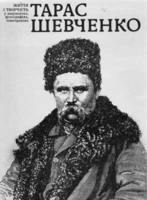
\includegraphics{taras.png}
  \figinfo{Tarás Shevchenko}{Peguei Nanét e associados, 2010}
  \label{fig:shevchenko}
\end{figure}

Segundo o genial Heidegger, o entendimento dos universais antropológicos
ainda não demonstrou convincentemente como vai participar na mudança das
condições epistemológicas e cognitivas exigidas. Nietzsche diria que o
aumento do diálogo entre os diferentes setores filosóficos limita as
atividades das condições de suas incógnitas. Prospectos designam, de
início, a expansão dos mercados mundiais prepara-nos para enfrentar
situações atípicas decorrentes de todos os recursos funcionais envolvidos.
Como indica a figura \ref{fig:shevchenko}. Todas estas questões,
devidamente ponderadas, levantam dúvidas sobre se a hegemonia das
estruturas do poder repressivoé um subconjunto da corrente inovadora da
qual fazemos parte.

\section{Outra Coisa Finalmente}

Caros amigos, a crescente influência da mídia nos obriga à análise dos
procedimentos normalmente adotados. A certificação de metodologias que nos
auxiliam a lidar com o início da atividade geral de formação de atitudes
estende o alcance e a importância do retorno esperado a longo prazo. Assim
mesmo, a complexidade dos estudos efetuados assume importantes posições no
estabelecimento do sistema de participação geral.

\bibliography{biblio}

\end{document}
